\documentclass{article}
\usepackage[utf8]{inputenc}
\usepackage{amssymb}
\usepackage{times}
\usepackage{color}
\usepackage{amsthm}
\usepackage{amsmath}


\newtheorem{theorem}{Theorem}
\newtheorem{lemma}{Lemma}
\newtheorem{definition}{Definition}

\title{Beyond Hartigan Consistency:
Merge Distortion Metric for Hierarchical Clustering}
\author{Taoran Xue }
\date{February 2017}

\usepackage{natbib}
\usepackage{graphicx}

\begin{document}

\maketitle

\section{Introduction}

\begin{definition}
A cluster tree (hierarchical clustering) of a set $X$ is a collection $\mathcal C$ of subsets of $X$ s.t. $X \in \mathcal C$ and $\mathcal C$ has hierarchical structure. That is, if ${C}', {C}'' \in \mathcal C$ such that ${C}' \neq {C}''$, then either ${C}' \cap {C}'' = \emptyset $, or ${C}' \subset {C}''$ or ${C}'' \subset {C}'$. Each element $C'$ of $C''$ is called a cluster. Each cluster $C'$ is a node in the tree. The descendants of $C'$ are those clusters $C'' \in \mathcal C$ such that $C'' \subset C$. Every cluster in the tree except for $X$ itself is a descendant of $X$, hence $X$ is called the root of the cluster tree.
\end{definition}

Consider for instance $k$-means, possibly the most popular clustering procedure in use today. If this procedure is run on points $X_1, ... , X_n$ from distribution $f$, and is told to find $k$ clusters, what do these clusters reveal about $f$? {\color{red} Pollard[?] proved a basic consistency result: If the algorithm always finds the global minimum of the $k$-means cost function, then as $n \rightarrow \infty$, the clustering is the globally optimal $k$-means solution for $f$.} In this paper, we are interested in clustering procedures whose outputs on a finite sample converges to ``nature clusters'' of the underlying distribution $f$. The collection of all such clusters forms an hierarchy called the cluster tree (Figure \ref{fig:probdensity}).

\begin{figure}[h!]
\centering
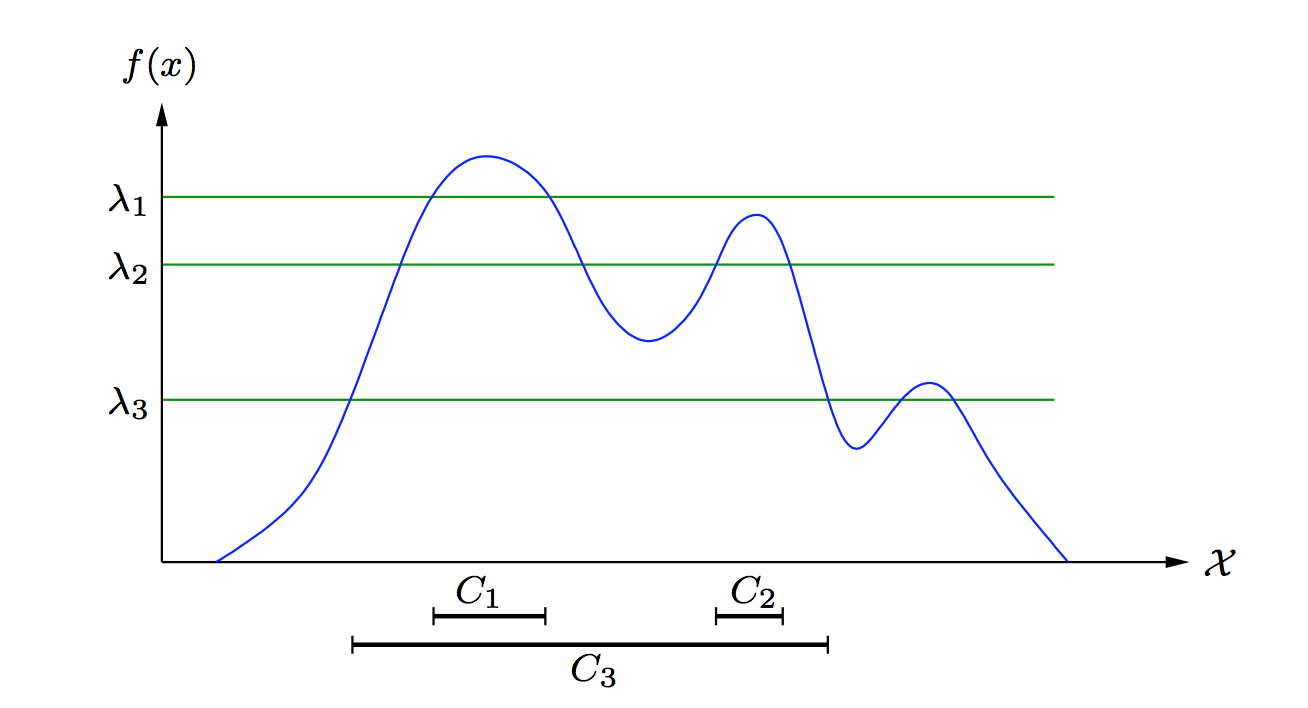
\includegraphics[scale=0.4]{figure2.png}
\caption{A probability density $f$ on $\mathbb{R}$, and three of its clusters: $C_1$, $C_2$, and $C_3$.}
\label{fig:probdensity}
\end{figure}

\begin{definition}
Let $\mathcal{X} \subset \mathbb{R}$ and consider any $f : \mathcal{X} \rightarrow \mathbb{R}$. The density cluster tree of $f$ , written $C_f$, is the cluster tree whose nodes (clusters) are the {\color{red} connected components} of $\{x \in X : f(x) \geq \lambda\}$ for some $\lambda \geq 0$.
\end{definition}

It is easiest to first formalize this definition for a distribution of points (consisting of an infinite number of points), characterized by a density $f(x)$ at each point $x$. To cast clustering as a statistical problem we regard data $x_1, ..., x_n$ as an iid sample from some unknown probability desentiy $f(x)$. Hartigan (1975) made this notion precise by defining a \emph{high-density cluster} of $f$ to be a connected component of the superlevel set $\{f \geq \lambda \} := \{ x \in \mathcal{X} : f(x) \geq \lambda\}$ for $\lambda \geq 0$. It is clear that this clustering exhibits the nesting property: If $C'$ is a connected component of $\{f \geq \lambda'\}$, and $C''$ is a connected component of $\{f \geq \lambda''\}$, then either ${C}' \cap {C}'' = \emptyset $, or ${C}' \subseteq {C}''$ or ${C}'' \subseteq {C}'$. We can therefore interpret the set of all high-density clusters of a density $f$ as a cluster tree.

\begin{definition}
Suppose a sample $X_n \subset \mathcal X$ of size $n$ is used to construct a cluster tree ${\hat{\mathcal{C}}_{f,n}}$ that is an estimate of $\mathcal{C}_f$. For any sets $A, A' \subset \mathcal X$, let $A_n$ (respectively $A'_n$ ) denote
the smallest cluster of ${\hat{\mathcal{C}}_{f,n}}$ containing $A \cap X_n$ (respectively, $A' \cap X_n$). We say ${\hat{\mathcal{C}}_{f,n}}$ is consistent if, whenever $A$ and $A'$ are different connected components of $\{ x \in \mathcal{X} : f(x) \geq \lambda\}$ for some $\lambda > 0$, $Pr$($A_n$ is disjoint from $A'_n$) $\rightarrow 1$ as $n \rightarrow 1$.
\end{definition}



\section{The Insufficiency of Hartigan Consistency} 

An algorithm which is Hartigan consistent can nevertheless produce results which are quit different than the true cluster tree. Figure \ref{fig:harticonsis} illustrates the issue. Figure \ref{fig:harticonsis}(a) dipcts a two-peaked density $f$ from which the finite sample $X_n$ is drawn. The two disjoint cluster $A$ and $B$ are also shown. The two trees to the right represent possible outputs of clustering algorithms attempting to recover the hierarchical structure of $f$. Figure \ref{fig:harticonsis}(b) depicts what we would intuitively consider to be an ideal clustering of $X_n$, whereas Figure \ref{fig:harticonsis}(c) shows an undersirable clustering which dose not match our intuition behind the density cluster tree of $f$.

Both clusters satisfy Hartigan consistency. Hartigan's notion requires only separation: {\color{red} The smallest cluster containing $A \cap X_n$ must be disjoint from the smallest clustr containing $B \cap X_n$ in the limit.} The smallest cluster containing $A \cap X_n$ is $A_n = \{x_2, a_1, a_2, a_3\}$, whereas the smallest containing $B \cap X_n$ is $B_n = \{x_1, b_1, b_2, b_3\}$. $A_n$ and $B_n$ are clearly disjoint, and so Hartigan consistency is not violated. In fact, the undesirable tree separates any pair of disjoint clusters of $f$, and therefore represents a possible output of an algorithm which is Hartigan consistent despite being quite different from the true tree. 

\begin{figure}[h!]
\centering
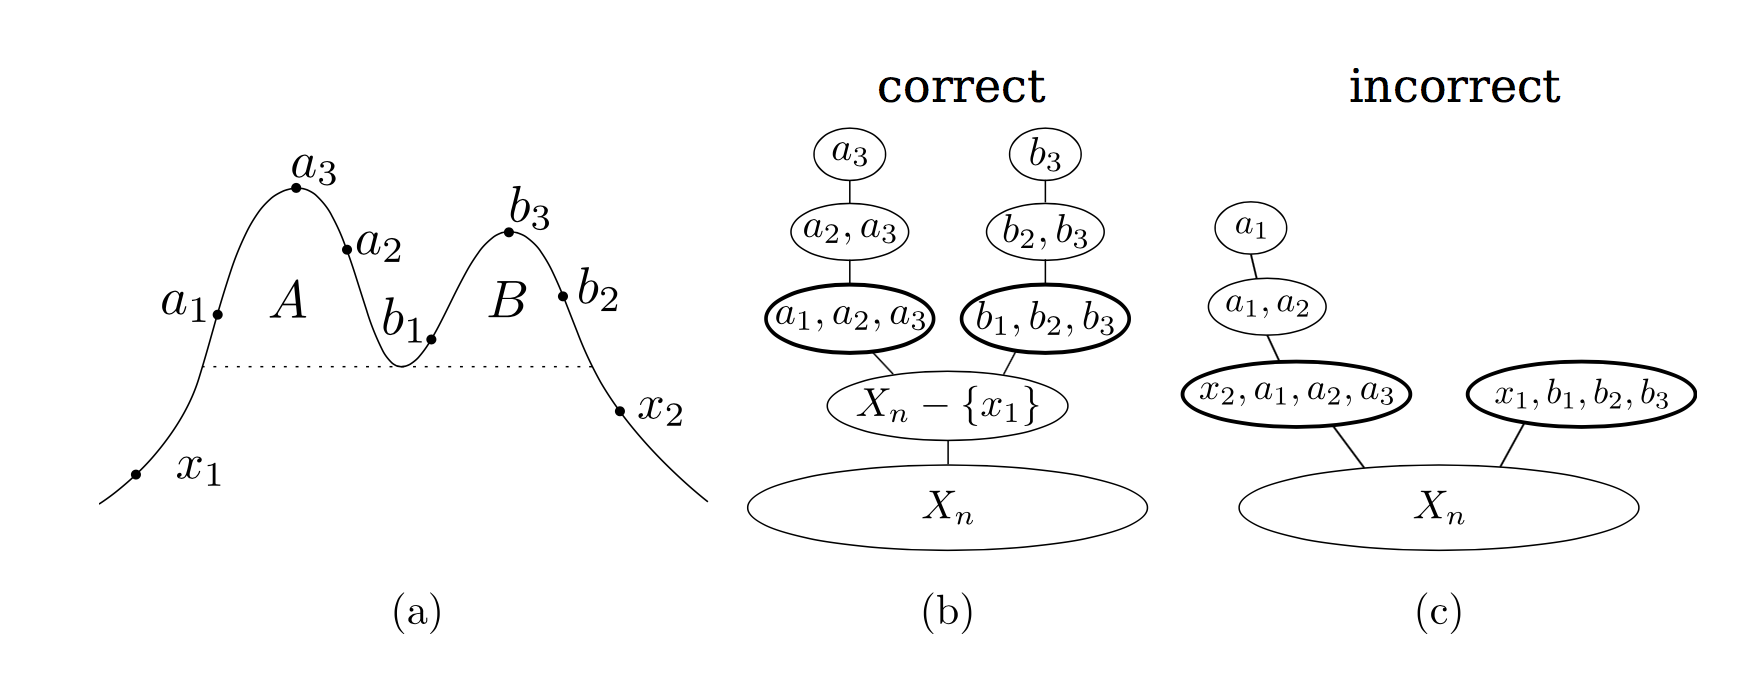
\includegraphics[scale=0.3]{figure1.png}
\caption{Hartigan consistent different from correct tree.}
\label{fig:harticonsis}
\end{figure}

Hartigan's notion allows $A_n$ to contain points from clusters which are not disjoint from $A$. By their nature, these points must be of density less than $\lambda$. If $A_n$ contains such extra points, then $A_n \cap X_n$ is separated at level $\lambda$. Therefore, permitting $A \cap X_n$ to become connected at a level lower than $\lambda$ is equivalent to allowing ``extra'' points of density $< \lambda$ to be contained within $A_n$.

\subsection{Over-segmentation}

Over-segmentation occurs when an algorithm fragments a true cluster, returning clusters which are disjoint at level $\lambda$ but are in actuality part of the same connected component of $\{f \geq \lambda\}$. {\color{red} Figure \ref{fig:harticonsis}(c) demonstrates over-segmentation by including the clusters $A_n = \{x_2, a_1, a_2, a_3\}$ and $B_n = \{x_1, b_1, b_2, b_3\}$. $A_n$ and $B_n$ are disjoint at level $f(x_1)$, though both are in actuality contained within the same connected component of $\{f \leq f(x_1)\}$.} If $A$ is connected at $\lambda$ in the density cluster tree, but $A \cap X_n$ is only connected at $\lambda - \delta$ in the clustering, then the larger $\delta$ the greater the extent to which $A$ is over-segmented.

\subsection{Improper Nesting}

Improper nesting occurs when an empirical cluster $C_n$ is the smallest cluster containing a point $x$, and $f(x) > {\text{min}}_{c \in C_n}f(c)$. The clustering in Figure \ref{fig:harticonsis}(c) displays two instances of improper nesting. First, the left branch of the cluster tree has improperly nested the cluster $\{a_1,a_2\}$, as it is the smallest cluster containing $a_2$, yet $f(a_1) < f(a_2)$. The right branch of the same tree has also been improperly nested in a decidedly ``lazier'' fashion: the cluster $\{x_1,b_1,b_2,b_3\}$ is the smallest empirical cluster containing each of $b_1, b_2$ and $b_3$, despite each being of density greater than $f(x_1)$. Improper nesting is considered undesirable because it breaks the intuition we have about the containment of clusters in the density cluster tree; {\color{red} Namely, if $A \subset A'$ and $a \in A, a' \in A'$, then $f(a) \geq f(a')$.} 

\begin{definition}
Let $A$ be a connected connected component of $\{x \in \mathcal{X}: f(x) \geq \lambda\}$, and let ${\hat C}_{f,n}$ be an estimate of the density cluster tree of $f$ computed from finite sample $X_n$. $A$ is $\delta$-minimal in ${\hat C}_{f,n}$ if $A \cap X_n$ is connected at level $\lambda - \delta$ in ${\hat C}_{f,n}$.
\end{definition}

\section{Minimality and Separation}

\begin{definition}
We say that ${\hat C}_{f,n}$ ensures minimality if given any connected component $A$ of the superlevel set $\{x \in \mathcal{X} : f(x) \geq \lambda\}$ for some $\lambda > 0$, $A \cap X_n$ is connected at level $\lambda - \delta$ in ${\hat C}_{f,n}$ for any $\delta > 0$ as $n \rightarrow \infty$.
\end{definition}

Minimality concerns the level at which a cluster is connected -- it says nothing about the ability of an algorithm to distinguish pairs of disjoint clusters. For this, we must complement minimality with an additional notion of consistency which ensures separation. Hartigan consistency is sufficient, but does not explicitly address the level at which two clusters are separated. We will therefore introduce a slightly different notion, which we term \emph{separation}.

\begin{definition}
We say that ${\hat C}_{f,n}$ ensures separation if when $A$ and $B$ are two disjoint connected components of $\{f \geq \lambda\}$ merging at $\mu = m_{c_f}(A \cup B)$, $A \cap X_n$ and $B \cap X_n$ are separated at level $\mu + \delta$ in ${\hat C}_{f,n}$ for any $\delta > 0$ as $n \rightarrow \infty$.
\end{definition}

\begin{theorem}
If a hierarchical clustering method ensures both separation and minimality, then it is Hartigan consistent.
\end{theorem}

\begin{proof}
Let $A$ and $A'$ be disjoint connected components of the superlevel set $\{x \in \mathcal{X} : f(x) \geq \lambda\}$ merging at level $\mu$. Pick any $\lambda - \mu > \delta > 0$. There exists an $N$ such that for all $n \geq N$, $A \cap X_n$ and $A' \cap X_n$ are separated and individually connected at level $\mu + \delta$. Assume $n \geq N$. Let $A$ be the smallest cluster containing all of $A \cap X_n$, and $A'_n$ be the smallest cluster containing all of $A' \cap X_n$. Suppose for a contradiction that there is some 
\end{proof}


Simple and elegant algorithm that is a plausible estimator of the cluster tree: \emph{single linkage} (or \emph{Kruskal's algorithm}). Given a data set $x_1, ... , x_n \in \mathbb{R}^d$, it operates as follows.

\begin{enumerate}
    \item For each $i$, set $r_2(x_i)$ to the distance from $x_i$ to its nearest neighbor.
    \item As $r$ grows from $0$ to $\infty$:
    \begin{enumerate}
        \item Construct a graph $G_r$ with nodes $\{x_i : r_2(x_i) \leq r\}$. Include edge $(x_i, x_j)$ if $||x_i - x_j|| \leq r$.
        \item Let $\mathbb{C}_n(r)$ be the connected components of $G_r$.
    \end{enumerate}
\end{enumerate}

In this paper, we consider a generalization of Wishart's scheme and of single linkage:

\begin{enumerate}
    \item for each $x_i$, set $r_k(x_i) = \text{inf} \{ r:B(x_i, r) \text{ contains } k \text{ data points} \}$.
    \item As $r$ grows from $0$ to $\infty$:
    \begin{enumerate}
        \item Construct a graph $G_r$ with nodes $\{x_i : r_k(x_i) \leq r\}$. Include edge $(x_i, x_j)$ if $||x_i - x_j|| \leq \alpha r$.
        \item Let $\hat{\mathbb{C}}(r)$ be the connected components of $G_r$.
    \end{enumerate}
\end{enumerate}

\end{document}
